\documentclass[12pt]{article}
\usepackage{tikz}
\usepackage{amsmath}
% Underlining package
\usepackage{ulem}
\usetikzlibrary{calc}
\usepackage[a4paper, portrait, margin=1cm]{geometry}
\usepackage{fancyhdr}

\def \HeadingQuestions {\section*{\Large Name: \underline{\hspace{8cm}} \hfill Date: \underline{\hspace{3cm}}} \vspace{-3mm}
{Coordinates: Questions} \vspace{1pt}\hrule}

% raise footer with page number; no header
\fancypagestyle{myfancypagestyle}{
  \fancyhf{}% clear all header and footer fields
  \renewcommand{\headrulewidth}{0pt} % no rule under header
  \fancyfoot[C] {\thepage} \setlength{\footskip}{14.5pt} % raise page number allowed min 14.5pt
}
\pagestyle{myfancypagestyle}  % apply myfancypagestyle

\newcounter{minipagecount}

\begin{document}
\HeadingQuestions

\bigskip
Plot the following points on the coordinate plane:

\[
\begin{array}{lllll}
A(9, -2) \quad & B(-9, -8) \quad & C(-4, -10) \quad & D(0, 4) \quad & E(-5, -6) \\
F(-6, 5) \quad & G(-1, 9) \quad & H(3, -9) \quad & I(8, 2) \quad & J(-7, -3) \\
\end{array}
\]

\bigskip

\begin{center}
  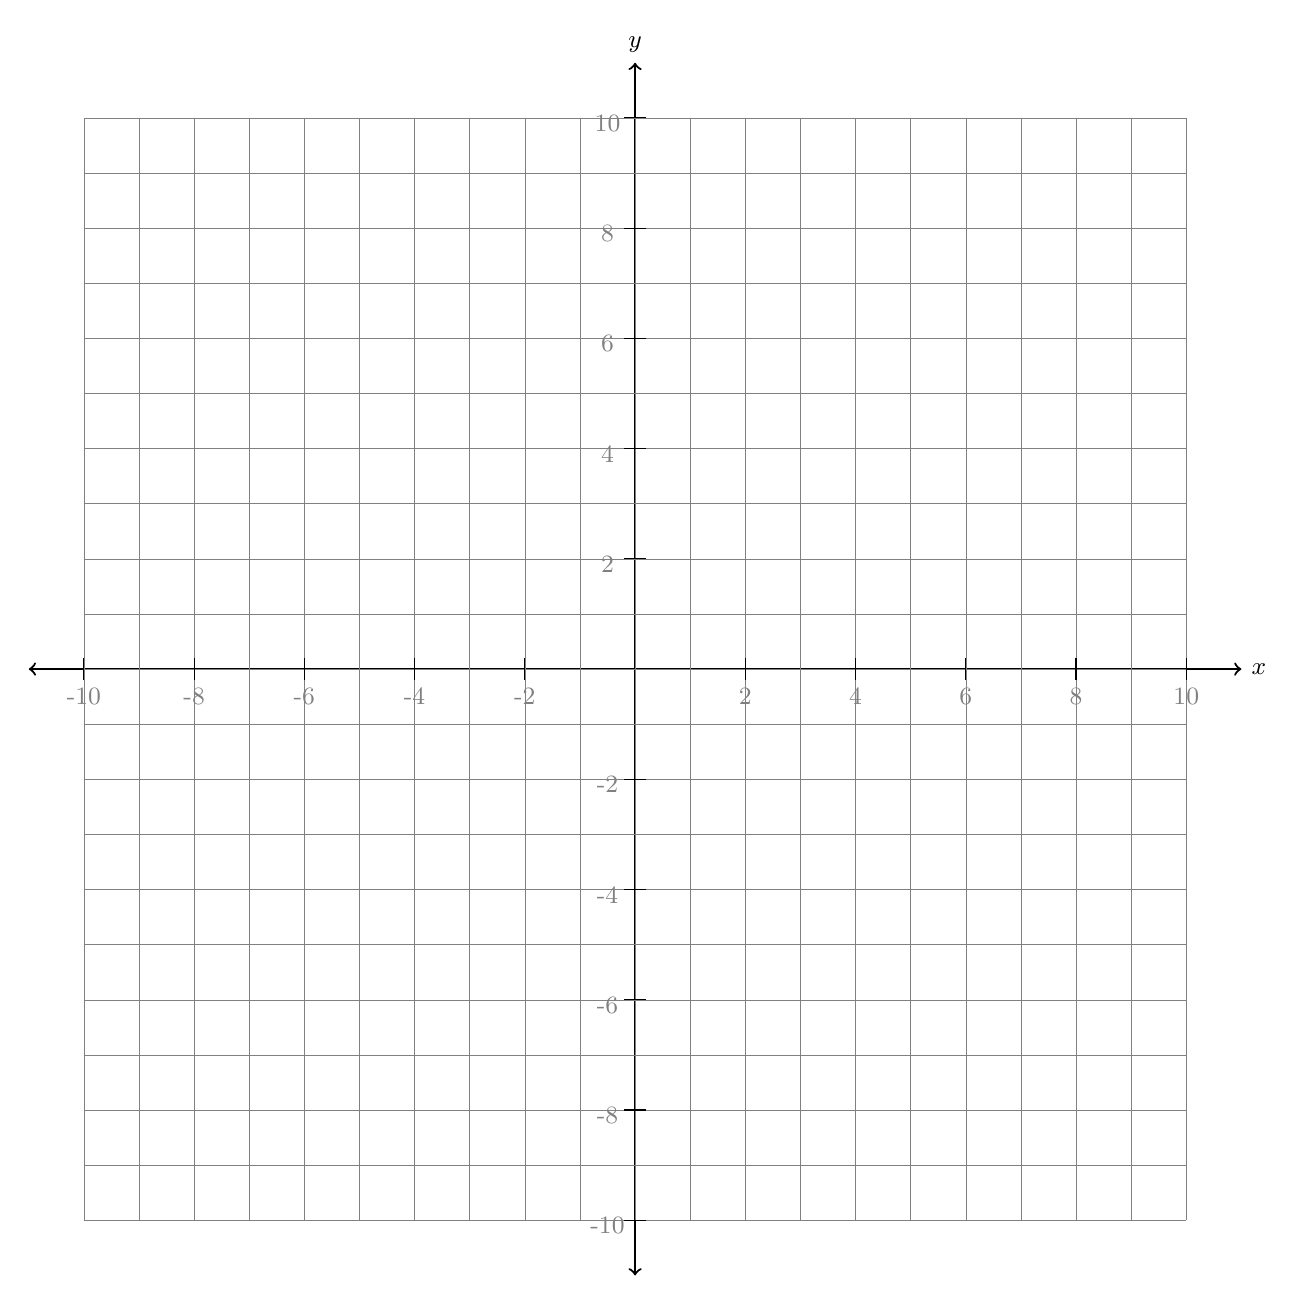
\begin{tikzpicture}[scale=0.7]
      % Draw axes
      \draw[thick,<->] (-11,0) -- (11,0) node[right] {\small $x$};
      \draw[thick,<->] (0,-11) -- (0,11) node[above] {\small $y$};

      % Grid
      \draw[very thin,gray] (-10,-10) grid (10,10);

      % Axis numbering (every second number, light gray)
      \foreach \x in {-10,-8,-6,-4,-2,2,4,6,8,10} {
          \draw (\x,-0.2) -- (\x,0.2);
          \node[gray] at (\x,-0.5) {\small \x};
      }
      \foreach \y in {-10,-8,-6,-4,-2,2,4,6,8,10} {
          \draw (-0.2,\y) -- (0.2,\y);
          \node[gray] at (-0.5,\y-0.1) {\small \y};
      }

    

  \end{tikzpicture}
\end{center}

\end{document}
